\section{Border Router Realization}

\subsection{Introduction}
In Thread when the users want to access their networks it is only possible if they have a gateway between the Thread and non-Thread network. This section will show a possible solution for this device. The gateway or \textit{Border Router} can be implemented with a \textit{Co-Processor}. Nordic, Zephyr and the OpenThread provides solutions for this. Here, it is important to get familiar with two types of concepts in the world of Co-Processors.
\begin{figure}[!htb]
    \centering
    \subfigure[Network Co-Processor]{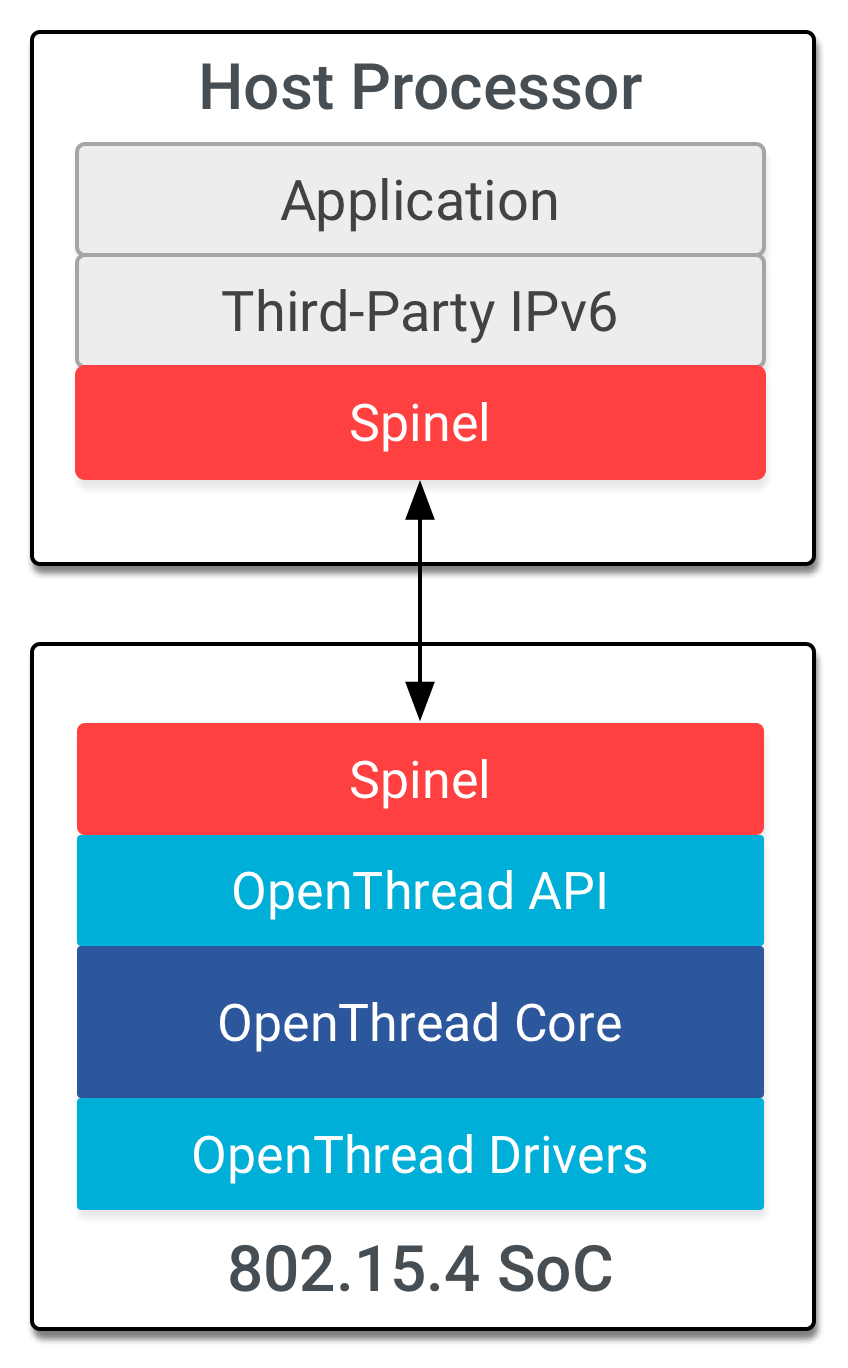
\includegraphics[width=5cm]{img/ncp-design.png}}
    \hfill
    \subfigure[Radio Co-Processor]{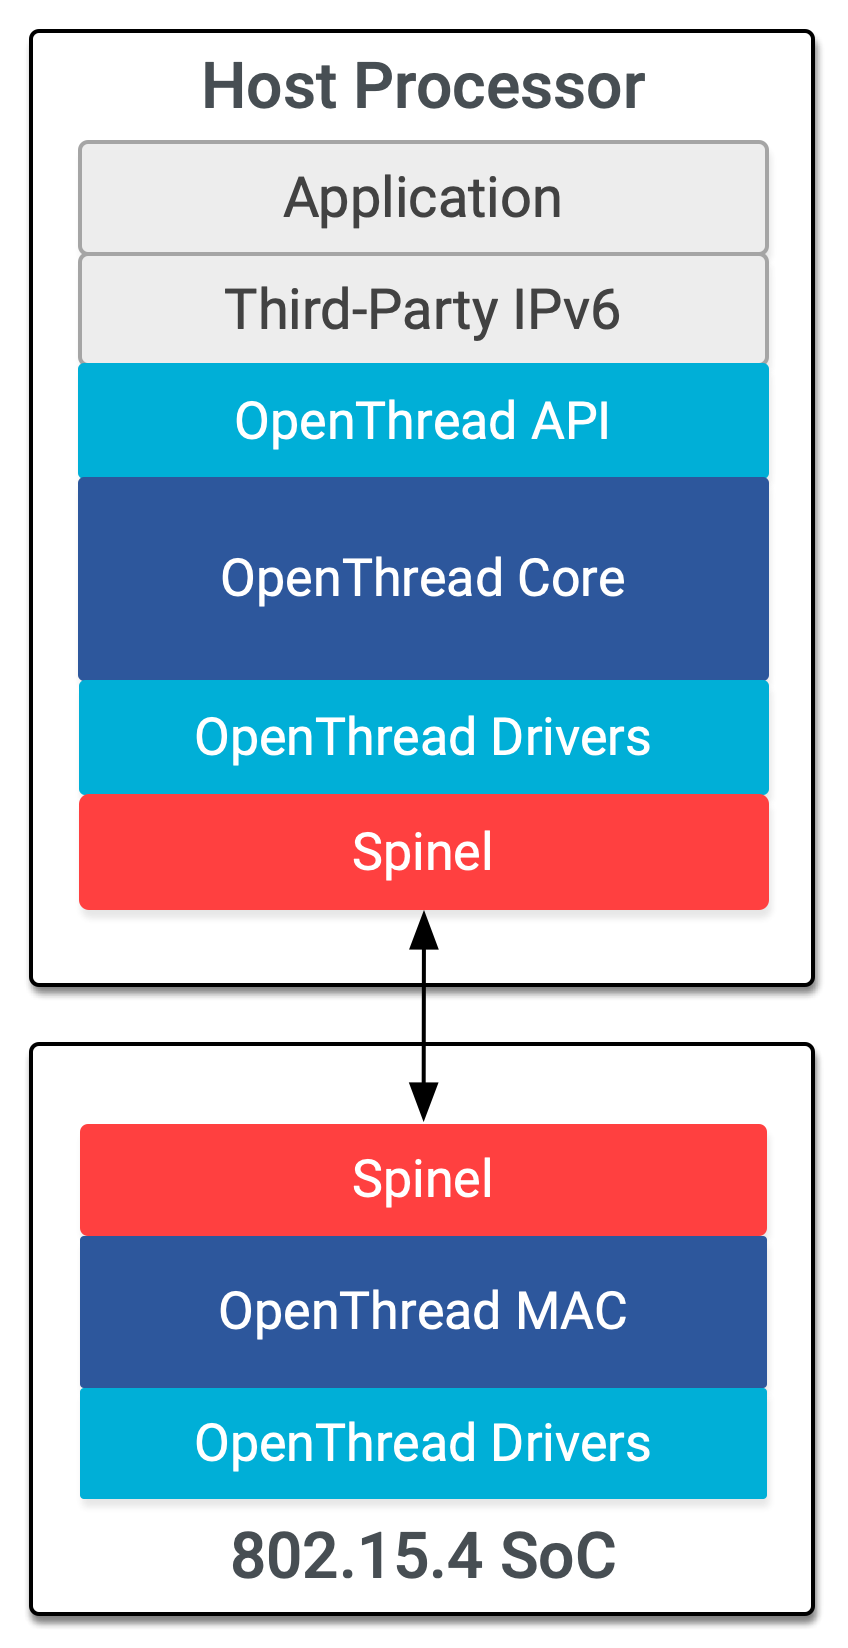
\includegraphics[width=5cm]{img/rcp-design.png}}
    \caption{Network Co-Processor vs. Radio Co-Processor}
    \label{fig:ncp}
    \cite{platforms}
\end{figure}

\subsubsection{Network Co-Processor}
One of these solutions is the \textit{Network Co-processor} (\textbf{NCP}), which is shown on the left side of the Figure \ref{fig:ncp}. The developers are using this design, when offload of the main resource (\textit{Host processor}) is required to save energy, as it allows to run the processor in \textit{idle} state or even keep it asleep. It may also be the case that some resource-intensive activity makes it important not to overload the processor, such as processing an image from a camera. In this case, the Thread API and the layer needed to construct the communication principle (\textit{Thread Core}) will run together with the physical layer of the Thread Radio on a much lower power, separate processor. The Host processor and the Co-Processor can communicate via UART, SPI or USB. In the diagram, this communication is implemented in the "Spinel" layer, which is a protocol developed by Google specifically for this task. This protocol is described in this \href{https://datatracker.ietf.org/doc/html/draft-rquattle-spinel-unified}{documentation}\cite{SpinelDoc}. From the image on the left, it can be concluded that the Host will only run IPv6 management and the application.

\subsubsection{Radio Co-Processor}
In this case, which called \textit{Radio Co-Processor} (\textbf{RCP}), only a minimal communication layer of Thread MAC and the physical driver are running together. This has the advantage that all OpenThread-related layers are located on the much more powerful Host processor. The biggest benefit is, when the Thread API or Thread core changes, the device is not needed to flash with the new firmware. As in the previous case, it communicates via some sort of serial communication.

\subsection{The Co-Processor design used for the implementation}
Based on the above, I created my own Border Router using NCP in the first version, but due to the continuous rapid changes in OpenThread, a direction is emerging that the RCP design will prevail in the development phase. It is currently the only one supported by Google, so I have continued development and hardware design in that direction. 

\subsection{Raspberry Pi HAT - Border Router}
\subsubsection{Requirements}
I created the Border Router with a Raspberry Pi 4 and on it a self designed and programmed HAT. The word \textbf{HAT} comes from \textit{Hardware Attached on Top}. Since 2014, Raspberry Pi has been developing the HATs \href{https://github.com/raspberrypi/hats}{GitHub}\cite{HATSGitHub} repository. The idea behind which is to create different devices using the Raspberry Pi Model B pin header. This consists of 40 pins since the second series and its basic layout has not changed since then. Over the years, as more and more complex Broadcom chips appear in the Raspberry, more and more functions are available on a single pin header's pin. On these HATs if I place an EEPROM, which is communicating via I2C, than the Raspberry Pi can configure the GPIO pins at boot time based on the data in this memory.
It is a basic requirement that two pins (GPIO 0 and GPIO 1) dedicated to the I2C EEPROM can not be used for any other task. Furthermore, two other basic requirements are set by the developers. One is that if it is possible to connect the power supply from the HAT, it must be protected from back powering by an \textit{ideal diode}. If the power supply is connected through the Raspberry's power port, it can cause damage to the power module because of the different voltage levels. The third basic requirement is that certain pins must be protected from short-circuiting, as these are configured to output during boot time in older versions, as they are used for boot time signalling.
A device can only be described as a HAT if:
\clearpage
\begin{itemize}
    \item it satisfies the three basic requirements,
    \item it has an I2C EEPROM containing real, processable data and this is soldered on the HAT,
    \item it can connect to the Raspberry with a 40 pin spike line,
    \item it must follow the mechanical specification (given size and hole diameters),
    \item it has at least 8 mm distance between the two PCBs,
    \item it is capable of supplying at least 1.3\,\si{\ampere} of continuous current through the 5\,\si{\volt} pin.
\end{itemize}
During the design process I followed these guidelines, therefore my Thread Border Router could be called a HAT.

\subsubsection{EEPROM and stored data}
For EEPROM I chose a 256 \si{\kilo}Byte memory from OnSemiconductor\newline \textbf{CAT24Cxx}, because it has hardware write protection for the entire memory area, unlike the same series of ICs from Microchip. Thus, on the custom hardware a jumper must be removed when writing, so that the user can not accidentally overwrite the EEPROM contents.
This repository contains target-specific programs for writing EEPROM and generating EEPROM contents. To make configuration easier, it is needed to specify in a text file which GPIO pin and which function want to be configured, which can be input, output or an alternative function. These can be found in the documentation of the specific Raspberry Pi BCM chip. Furthermore, it is possible to add pull-ups or pull-downs to the input configured pins.
\begin{figure}[!htb]
    \centering
    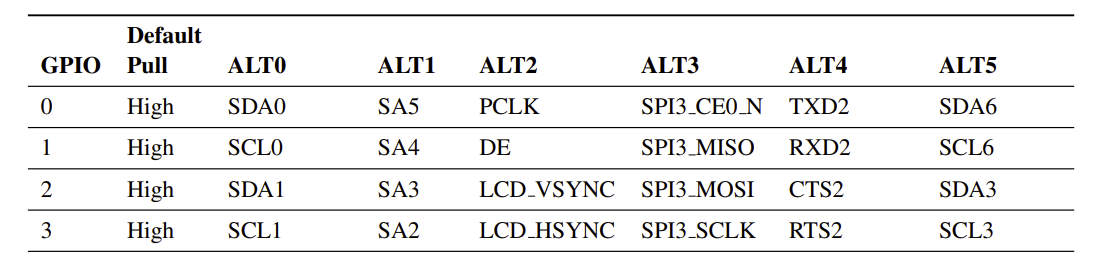
\includegraphics[width=\textwidth]{img/bcmgpio.png}
    \caption{The first four GPIO functions of the Raspberry Pi 4}
    \label{fig:gpios}
    \cite{RaspberryBCM}
\end{figure}
The Raspberry Pi 4 is built with a BCM2711 chip and the functions of the first four GPIO pins are shown in Figure \ref{fig:gpios}. From this table, it can be seen that if these are configured as ALT0 function pins, two I2C peripherals are obtained. In the other case, if an UART peripheral is needed with data flow control, it should be chosen to be ALT4 function.
If the memory is filled with valid data, the next time during the boot process of the Raspberry the data will be automatically read and the pins are initialized accordingly. It is important to note that there is a config.txt file in the \textit{/boot} partition where special peripherals are needed to be enabled with a program, which called \textit{dtoverlay}. For example, the dtoverlay program can enable the uart3 peripheral with flow-control with this line:
\begin{center}
    dtoverlay=uart3, ctsrts
\end{center}


\subsection{Raspberry Pi HAT - Border Router Design}
\begin{figure}[!htb]
    \centering
    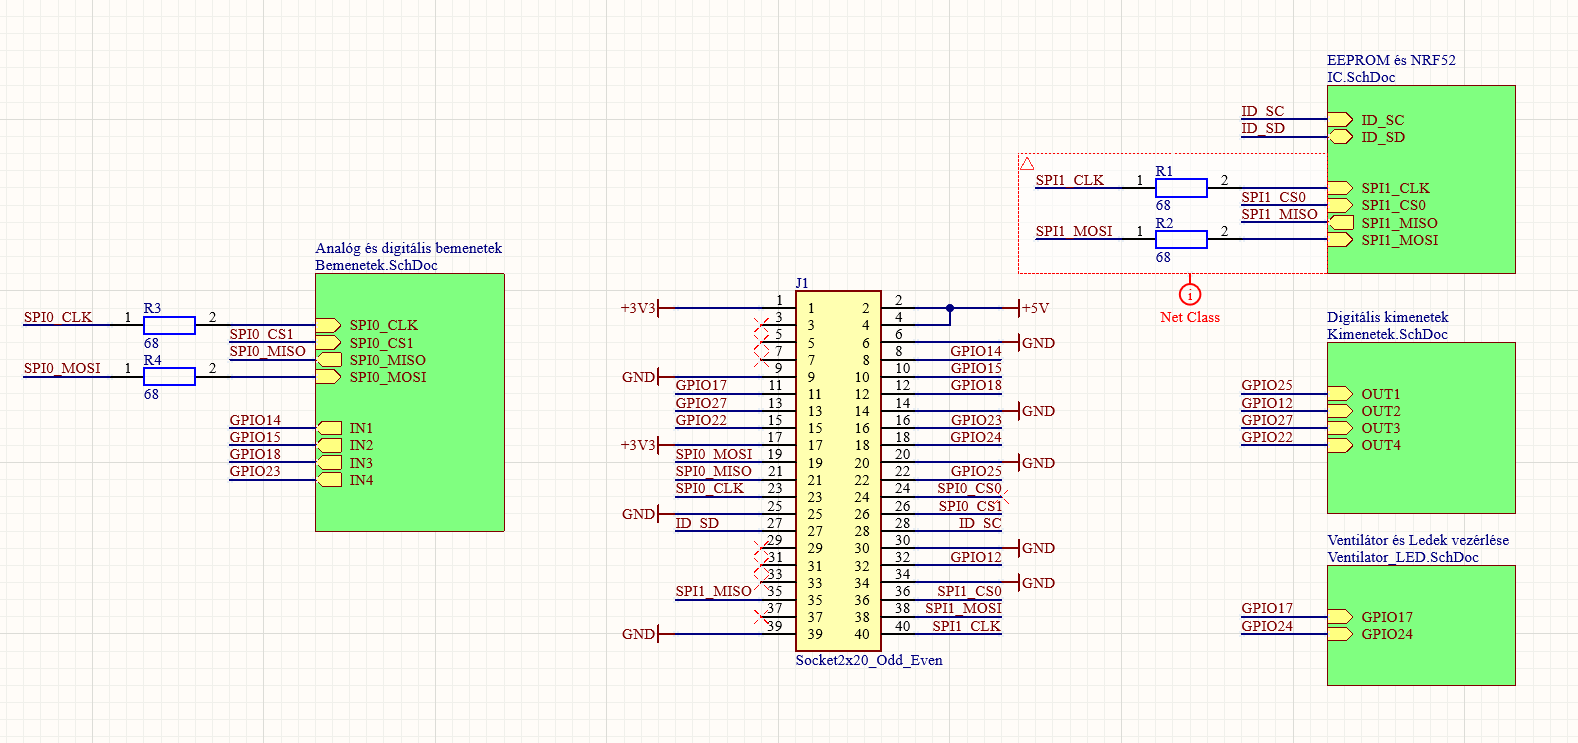
\includegraphics[width=\textwidth]{img/rpischematics.png}
    \caption{Raspberry Pi HAT wiring diagram}
    \label{fig:Schematics}
\end{figure}
\noindent
My goal was to develop a device that would be a transition between a Proof-Of-Concept and a final product. The hardware design was made with Altium Designer, because it is one of the most widely used design tool. As the Figure \ref{fig:Schematics} shows, the schematic can be divided into four different parts. Inputs are on the left side, where four digital and two analogue inputs are located. These inputs are protected against overvoltage (up to 7\,\si{\volt}), so that the digital inputs tolerates 5\,\si{\volt} TTL signals or in case of a bad connection the higher voltage can not damage the input/output pins. The analogue inputs measure the connected voltage in the range from 0 to 3.3\,\si{\volt}, thus offering additional applications. Since the Broadcom chip used by the Raspberry Pi does not have an analog-to-digital converter, the measurements are made by an external Microchip SPI-communicating IC for this, which was available compared to its I2C counterpart in the middle of the current chip shortage. In the middle there is the 40 pin socket and the connection for those. In the upper right corner the I2C EEPROM and an nRF52840 connected via SPI. To reduce the crosstalk, the design contains a 68 ohm resistor on each of the SCK and SDO lines to increase the rise/fall times of the changes. The digital outputs block is in the centre right, which have signal levels of 0 and 3.3\,\si{\volt} and are also protected from overvoltage and short circuit from connecting outputs due to bad wiring. The inputs, outputs, 5\,\si{\volt} and ground power lines are available through 50 mil grid spacing terminal blocks on the PCB. And in the lower right corner is shown the control block for the five LEDs and two fan outputs on the PCB. These can be switched on and off by 3.3\,\si{\volt} and the brightness and rotation speed can be controlled by PWM. The LEDs are for design purposes only, while the fans are used to protect the device from overheating. A detailed breakdown of the green blocks is shown in Figure \ref{fig:borderrouterbemenetek}-\ref{fig:borderventiled}.
\begin{figure}[!htb]
    \centering
    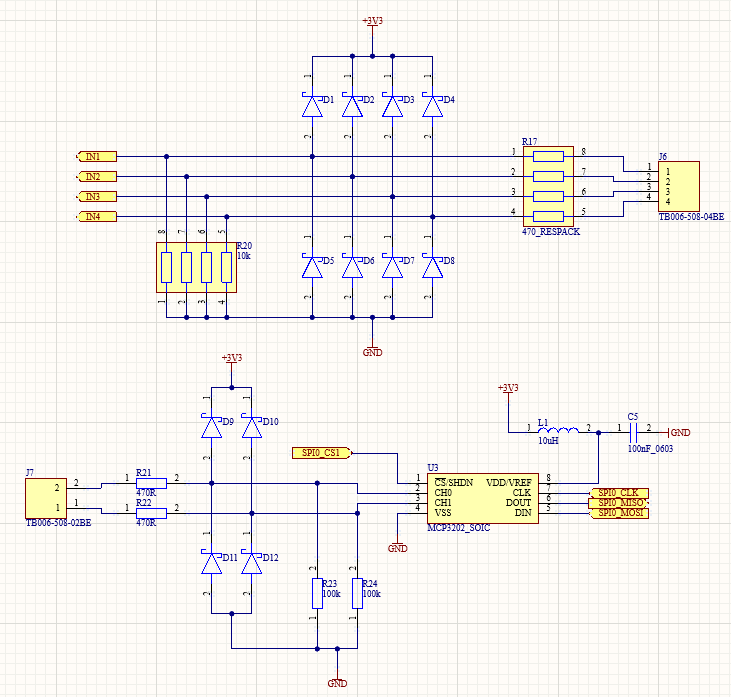
\includegraphics[width=\textwidth]{img/bemenetekrpihat.png}
    \caption{Raspberry Pi HAT inputs}
    \label{fig:borderrouterbemenetek}
\end{figure}
\begin{figure}[!htb]
    \centering
    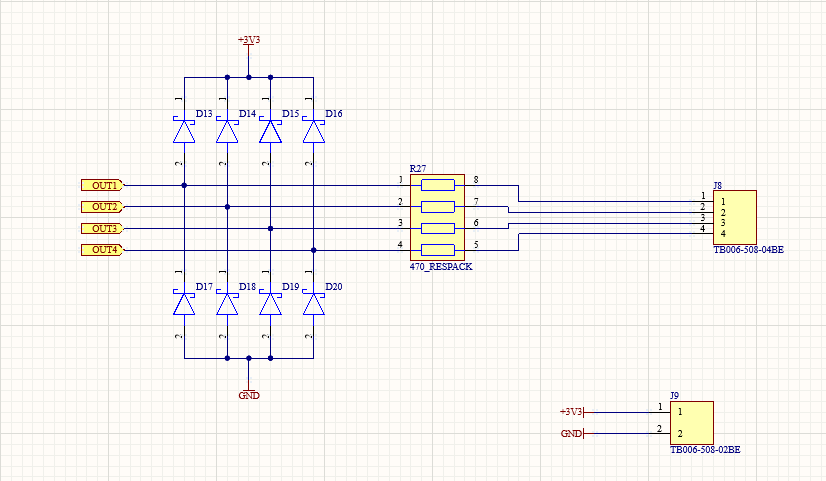
\includegraphics[width=\textwidth]{img/kimenetekrpi.png}
    \caption{Raspberry Pi HAT outputs}
    \label{fig:borderrouterkimenetek}
\end{figure}
\begin{figure}[!htb]
    \centering
    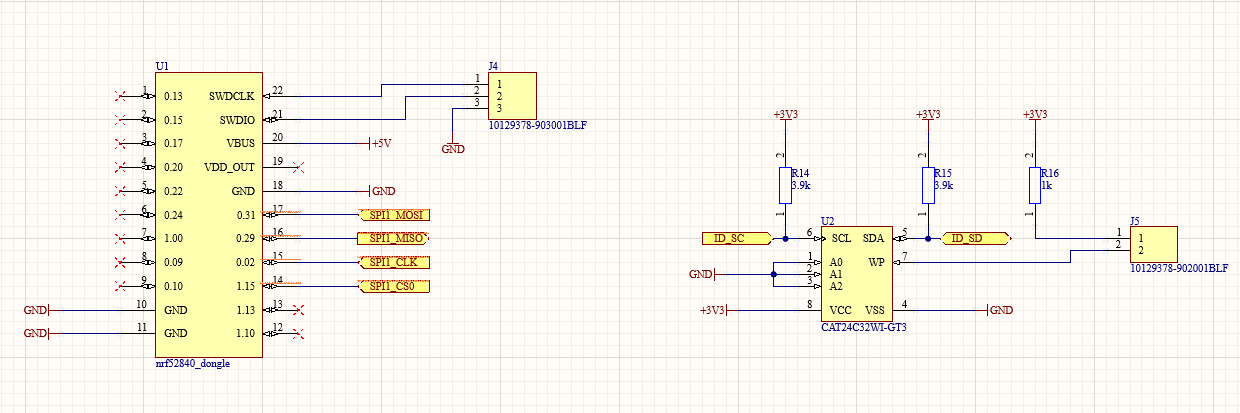
\includegraphics[width=\textwidth]{img/eeprom.png}
    \caption{Raspberry Pi HAT Integrated Circuits}
    \label{fig:borderrouterick}
\end{figure}
\begin{figure}[!htb]
    \centering
    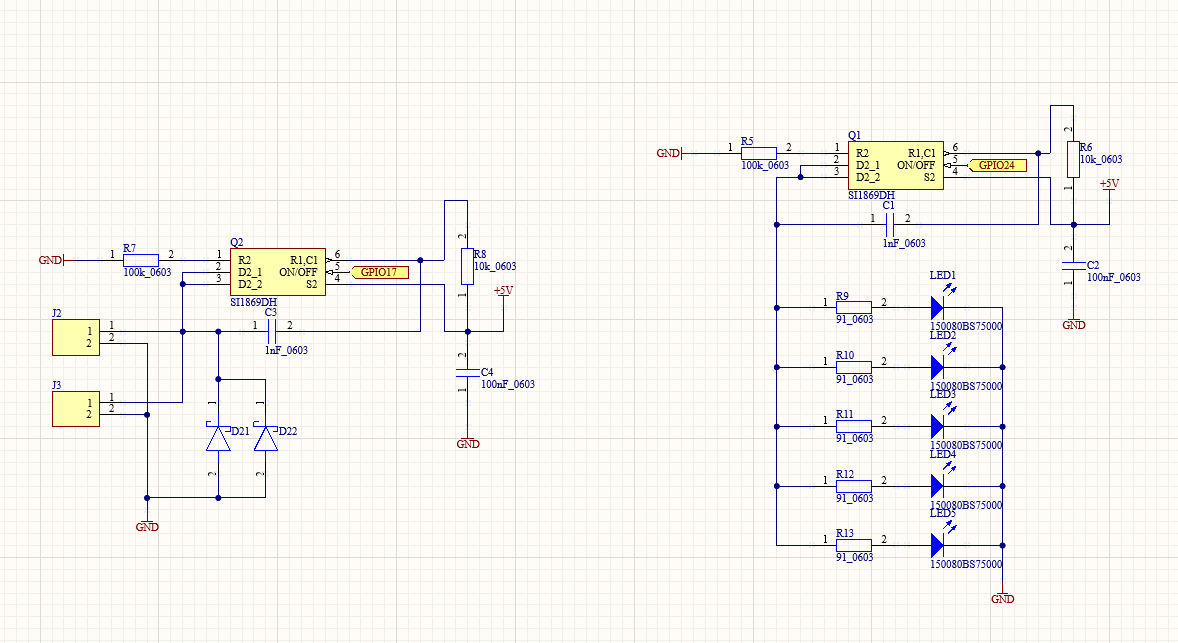
\includegraphics[width=\textwidth]{img/ickrpihat.png}
    \caption{Raspberry Pi HAT LED and fan controller}
    \label{fig:borderventiled}
\end{figure}
\newline
Figure \ref{fig:3drpi} shows the finished PCB plan in 3D view.
\begin{figure}[!htb]
    \centering
    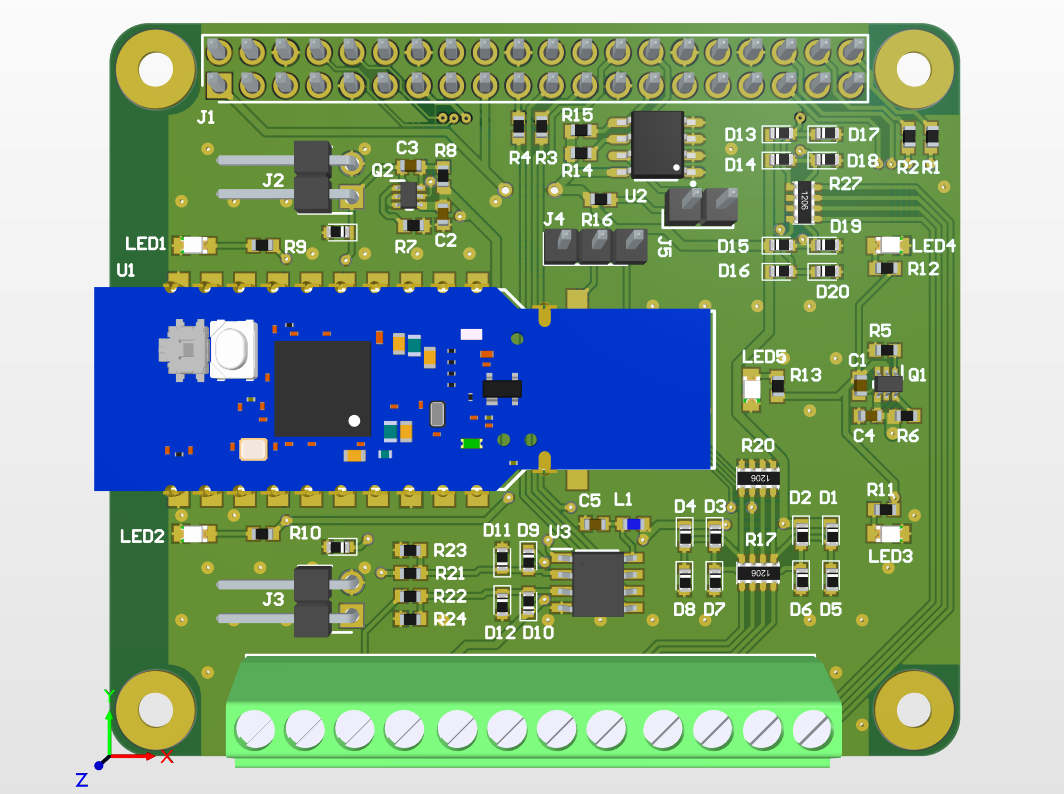
\includegraphics[width=\textwidth]{img/rpi3d.png}
    \caption{Raspberry Pi HAT in 3D viewer}
    \label{fig:3drpi}
\end{figure}


\subsection{Border Router housing}
It was important to make a housing in which I can place the Border Router, thus protecting the device from mechanical damage. The model of this device was made in AutoCAD Inventor.
The model includes two 5\,\si{\volt} brushless DC fans (short \textbf{BLDC}) to reduce the Raspberry Pi temperature by blowing air through the housing. The Ethernet and USB Type C ports is cut out, as the device can only be powered via USB port and the Ethernet port is the only way to connect to the home network. There is also space for access to the screw terminal ports, so the user can easily access the the 5\,\si{\volt} power supply, inputs and outputs with a flat-head screwdriver. On the Figure \ref{fig:3dbd} there is the housing model in 3D viewer.
\begin{figure}
    \centering
    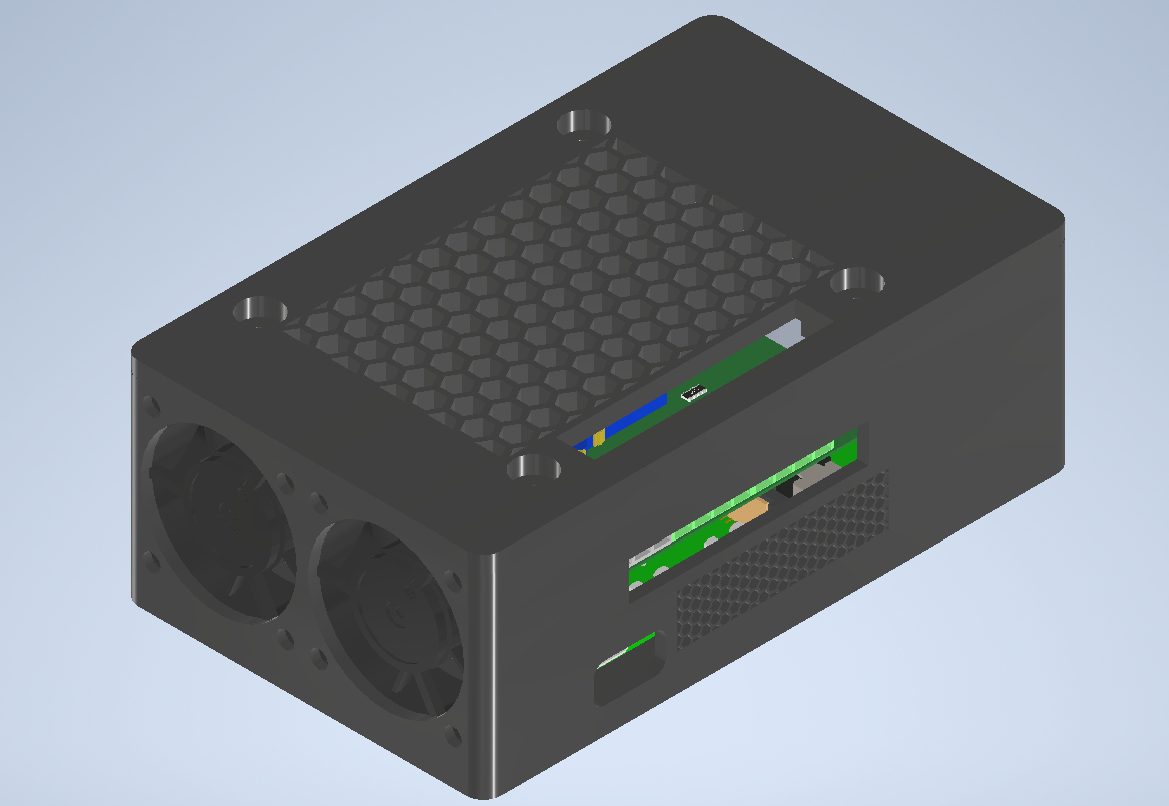
\includegraphics[width=\textwidth]{img/3ddoboz.png}
    \caption{Border Router housing in 3D viewer}
    \label{fig:3dbd}
\end{figure}


\subsection{Border Router software}
\subsubsection{nRF52840 RCP software}
For the Radio Co-Processor I use the package developed by OpenThread for nRF52840 and compiled it to the SPI pins. I modified the SPI pins in the dedicated header file, called "transport-config.h". The software is available at this \href{https://github.com/openthread/ot-nrf528xx}{GitHub repository}\cite{OTBR}. For the SPI communication, a total of six pins are required, four of for the SPI communication, one pin is tied to the hardware RESET pin of the microcontroller and one pin is held up for interrupt signalling. The last two pins are optional according to the documentation and if no interrupt signal is used, than the communication would be slowed down because the Host device would have to make continuous requests. In reality, the situation is different, since the code contains a section that if one of the two optional pins is missing, the program will return with an error code. Since the hardware RESET pin of the Dongle device is not hardwired, but is tied to a specific button, so SPI communication is not possible. So I switched to the much slower UART communication, which requires four pins, two data pins (Rx, Tx) and two signals (CTS, RTS). After uploading the code, the device was ready to communicate. It is worth noting that there are some pins that can only be used for low frequencies (10\,\si{\kilo\hertz}), as they run on-chip next to the RF module, so the manufacturer does not guarantee immunity to crosstalk.

\subsubsection{Raspberry Pi - OpenThread official software}
OpenThread provides a Raspbian-based GNU/Linux distribution to implement the the Border Router, but it is also available as a separate group of applications that the developer has to install. After the installations, three programs are available in the operating system, \textit{otbr-agent} (from OpenThread-BorderRouter name), which performs communication with the RCP via SPI, UART or USB, depending on the build. Closely related to this is the avahi-daemon, which resolves the Network Interfaces. The \textit{otbr-agent} makes a \textit{Wireless Personal Area} interface, namely \textbf{WPAN0}. If the \textit{ifconfig} program is used, than this program lists this interface in the result list. The third program is \textit{otbr-web}, which provides a configuration rudimentary web page at localhost address on port 80, where the user can create a Thread network, initiate a connection and view the before created Thread network with the available devices on this networks on a visualisation page. To connect an optional fourth program, which is called \href{https://github.com/openthread/ot-commissioner}{\textit{ot-commissioner}}\cite{OTCOMMISSIONER}, is required. Before use this have to be compiled, because this repository contains only the source code. Since the user or the developer can reach the Thread network over the internet via a website, this device act as a Border Router.

\subsubsection{Border Router scripts for other functions}
After boot time, when the otbr-agent software is available, I am using a Python script to create a Thread network by calling \textit{ot-cli}. With this program over the Linux kernel I can manage the Co-Processor, for example I can create my own Thread network, join an existing network or even map the network. A Python script manages the lights and the fan, that script constantly monitors the processor temperature and if it rises towards 60\,\si{\celsius}, the fan starts to spin up under the control of a 50\,\% duty cycle control signal. If it rises even further, the duty cycle changes on a linear scale up to 100\,\%, which is reached at 70\,\si{\celsius}.

\subsection{Summary of the Border Router}
In this section I presented the Border Router, which I designed. I showed the differences between NCP and RCP and the rules of HATs, which were necessary to develop this board. I showed the functionalities of this board and made a solution to set up a Thread network.